%\documentclass[xcolor=table,compress]{beamer}
\usepackage{etex}
%\documentclass{article}
%\usepackage{beamerarticle}
\usepackage{tikz} 
\usetikzlibrary{positioning,shapes,fit,arrows}
%\usepackage{pstricks,pst-node} % PSTricks package
%\usepackage[turkish]{babel}
\usepackage[utf8]{inputenc}
\usepackage{listings}
\usepackage{multicol}
%\includeonlyframes{current}

\mode<article>
{
  \usepackage{fullpage}
  \usepackage{pgf}
  \usepackage{hyperref}
}

\mode<presentation>
{
  \usetheme{metuceng}

  %\setbeamercovered{transparent}
}


\title{Programming Languages}
\subtitle{Values and Types}
\author{Onur Tolga Şehitoğlu}
\institute{Computer Engineering, METU}
\subject{Values and Types}
\date{}
	\titlegraphic{\insertmetutitle\insertlicense}


\begin{document}
\lstset{language=C,
        basicstyle=\scriptsize\ttfamily,
        keywordstyle=\color{blue!50!black}\bfseries,
        identifierstyle=\color{blue!60!green}\sffamily,
        stringstyle=\color{red!70!green}\ttfamily,
	commentstyle=\color{blue!30!white}\itshape,
        showstringspaces=true}
\setbeamercolor{hexample}{bg=green!5!white,fg=black}%
\setbeamercolor{cexample}{bg=blue!5!white,fg=black}%
\setbeamercolor{pexample}{bg=orange!5!white,fg=black}%

 \frame[plain]{\maketitle}
 \begin{frame}
 \frametitle{Outline}
 \small
 \begin{multicols}{2}
 \tableofcontents
 \end{multicols}
 \end{frame}

\section{Value and Type}
\begin{frame}
\frametitle{What are Value and Type?}
\begin{itemize}
 \item \structure{Value} anything that exist, that can be computed, stored, take part in data
 structure.\\
 	Constants, variable content, parameters, function return values, operator results...
\item \structure{Type} set of values of same kind.\\
	\pause C types:
	\begin{itemize}
		\item \texttt{int, char, long,...}
		\item \texttt{float, double}
		\item pointers
		\item structures: \texttt{struct, union}
		\item arrays
	\end{itemize}
\end{itemize}
\end{frame}

\begin{frame}
\begin{itemize}
\item Haskell types
\begin{itemize}
\item \texttt{Bool, Int, Float, ...}
\item \texttt{Char, String}
\item tuples,(N-tuples), records
\item lists
\item functions
\end{itemize}
\item Python types
\begin{itemize}
\item \texttt{bool, int, float, complex}
\item \texttt{str, bytes, tuple, list, set, dict}
\item classes, functions
\end{itemize}
\item Each type represents a set of values.
Is that enough?\\
\pause
What about the following set? Is it a type?\\
\texttt{\{"ahmet", 1 , 4 , 23.453, 2.32, 'b'\}} \pause
\item Values should exhibit a similar behavior. The \structure{same} group of operations
should be defined on them.
\end{itemize}
\end{frame}

\section{Primitive vs Composite Types}
\begin{frame}
 \frametitle{Primitive vs Composite Types}
\begin{itemize}
\item \structure{Primitive Types:} Values that cannot be decomposed into other sub values.\\
	C: \texttt{int, float, double, char, long, short}, pointers\\
	Haskell: \texttt{Bool, Int, Float}, function values\\
	Python: \texttt{bool, int, float, str}, functions
\item \structure{cardinality of a type:} 
The number of distinct values that a datatype has.
Denoted as: "\#Type".\\
\#Bool = 2 \ \ \#char = 256 \ \ \#short = $2^{16}$ \\
\#int = $2^{32}$ \ \ \#double = $2^{32}$, ...
\item What does cardinality mean?
\pause
How many bits required to store the datatype? 
\end{itemize}
\end{frame}

\begin{frame}
\frametitle{User Defined Primitive Types}
\begin{itemize}
\item \structure{enumerated types}\\
	\texttt{enum days \{mon, tue, wed, thu, fri, sat, sun\};\\}
	\texttt{enum months \{jan, feb, mar, apr,  .... }\};\\
\item \structure{ranges} (Pascal and Ada)\\
	\texttt{ type Day = 1..31; }\\
	\texttt{ var g:Day; }
\item \structure{Discrete Ordinal Primitive Types} Datatypes values have one to one mapping to
a range of integers.\\
C: Every ordinal type is an alias for integers.\\
Pascal, Ada: distinct types
\item DOPT's are important as they\\
	i. can be array indices, \texttt{switch/case} labels\\
	ii. can be used as \texttt{for} loop variable (some languages like pascal)
\end{itemize}
\end{frame}

\begin{frame}
\frametitle{Composite Datatypes}
User defined types with composition of one or more other datatypes. Depending
on composition type:
\begin{itemize}[<+->]
\item Cartesian Product (struct, tuples, records)
\item Disjoint union (union (C), variant record (pascal), Data (haskell))
\item Mapping (arrays, functions)
\item Powerset (set datatype (Pascal))
\item Recursive compositions (lists, trees, complex data structures)
\end{itemize}
\end{frame}

\section{Cartesian Product}
\begin{frame}
 \frametitle{Cartesian Product}
\begin{itemize}
\item $S \times T = \{ (x,y) \mid x \in S, y \in T \}$
\item Example:\\
$S=\{ a, b, c\} \;\;\; T=\{ 1, 2 \}$\\
$S \times T = \{ (a,1), (a,2), (b,1), (b,2), (c,1), (c,2) \}$\\
%\begin{pspicture}(0,0)
%\psframebox[linecolor=blue!50!black,framearc=1.5]{%
%	\begin{tabular}{l}$\bullet $a\\$\bullet $b\\$\bullet $c\end{tabular}} $\times$
%\psframebox[linecolor=blue!50!black,framearc=1.5]{%
%	\begin{tabular}{l}$\bullet $1\\$\bullet $2\end{tabular}} = 
%\psframebox[linecolor=blue!50!black,framearc=.8]{%
%	\begin{tabular}{l}$\bullet $(a,1)\ \ $\bullet $(a,2)\\\ 
%	$\bullet $(b,1)\ \ $\bullet $(b,2)\\
%	 	$\bullet $(c,1)\ \ $\bullet $(c,2)
%	\end{tabular}}
%\end{pspicture}
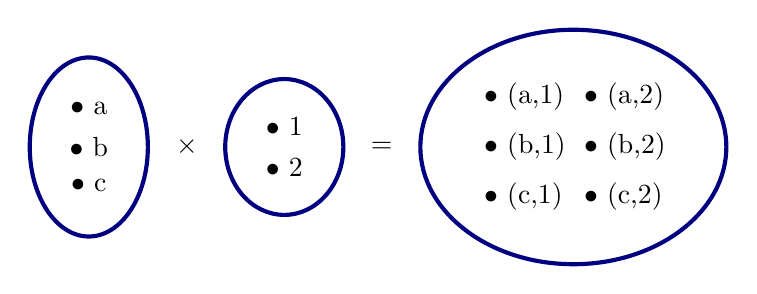
\begin{tikzpicture}
[node distance=5mm,  
 set/.style={line width=1.5pt, shape=ellipse, draw=black!50!blue}]
\matrix [row sep=.5mm] (setA)
{\node (aa) {$\bullet $ a} ; \\
\node  (ab) {$\bullet $ b}; \\
\node  (ac) {$\bullet $ c};\\
};
\node[set,minimum size=1.5cm,fit={(aa) (ac)}] {};
\node [right=of setA] (times) {$\times$};
\matrix [row sep=.5mm, right=of times] (setB)
{\node (b1) {$\bullet $ 1} ; \\
\node  (b2) {$\bullet $ 2}; \\
};
\node[set,minimum size=1.5cm,fit={(b1) (b2)}] {};
\node [right=of setB] (equal) {$=$};
\matrix [row sep=.5mm, right=of equal, xshift=3mm, ampersand replacement=\&] {
\node  (ca1) {$\bullet$ (a,1)}; \& \node {$\bullet$ (a,2)};\\
\node  {$\bullet$ (b,1)}; \& \node {$\bullet$ (b,2)};\\
\node  {$\bullet$ (c,1)}; \& \node (cb2){$\bullet$ (c,2)};\\
};
\node[set,minimum size=1.5cm,fit={(ca1) (cb2)}] {};
\end{tikzpicture}
\item $\#(S \times T) = $\pause $\#S \cdot \#T$
\end{itemize}
\end{frame}


\begin{frame}[fragile]
\begin{itemize}
\item C {\tt struct}, Pascal {\tt record}, functional languages \structure{tuple}
\item \textbf{in C:} string $\times$ int
\begin{beamercolorbox}{cexample}
\begin{lstlisting}[language={C}]
struct Person {
     char name[20];
     int no;
} x = {"Osman Hamdi",23141};
\end{lstlisting}\end{beamercolorbox}
\item \textbf{in Haskell}: string  $\times$ int 
\begin{beamercolorbox}{hexample}
\begin{lstlisting}[language={Haskell}]
type People=(String,Int)
...
x = ("Osman Hamdi",23141)::People
\end{lstlisting}
\end{beamercolorbox}
\item \textbf{in Python}: string $\times$ int
\begin{beamercolorbox}{pexample}
\begin{lstlisting}[language=python]
x = ( "Osman Hamdi", 23141)
type(x)
<type 'tuple'>
\end{lstlisting}
\end{beamercolorbox}
\end{itemize}
\end{frame}

\defverbatim[colored]\codecartC{%
\begin{lstlisting}[language={C}]
struct Person {
     char name[20];
     int no;
     enum Sex {MALE, FEMALE} sex;
} x = {"Osman Hamdi",23141,FEMALE};
\end{lstlisting}}
\defverbatim[colored]\codecartH{%
\begin{lstlisting}[language={Haskell}]
x = ("Osman Hamdi",23141,3.98,"Yazar")
\end{lstlisting}}

\begin{frame}[fragile]
\begin{itemize}
 \item Multiple Cartesian products:\\
C: string $\times$ int $\times$ \{MALE,FEMALE\}
\begin{beamercolorbox}{cexample}
 \codecartC
\end{beamercolorbox}\\
Haskell: string $\times$ int $\times$ float $\times$ string
\begin{beamercolorbox}{hexample}
 \codecartH
\end{beamercolorbox}\\
Python: str $\times$ int $\times$ float $\times$ str
\begin{beamercolorbox}{pexample}
\begin{lstlisting}[language=python]
x = ("Osman Hamdi",23141,3.98,"Yazar")
\end{lstlisting}
\end{beamercolorbox}
\end{itemize}

\end{frame}

\defverbatim[colored]\codehomC{%
\begin{lstlisting}[language={C}]
struct quad { double x,y,z,q; };
\end{lstlisting}}

\begin{frame}
\frametitle{Homogeneous Cartesian Products}
\begin{itemize}
 \item $S^n = \overbrace{S \times S \times S \times ... \times S}^{n}$\\
double$^4$ :
\begin{beamercolorbox}{cexample}
\codehomC 
\end{beamercolorbox}
\item $S^0 = \{ () \}$ is \structure{0-tuple}.
\item \alert{not} empty set. A set with a single value.
\item terminating value (nil) for functional language lists.
\item C \texttt{\structure{void}}. Means no value. Error on evaluation.
\item Python: \texttt{ () } . \lstinline!None! used for no value.
\end{itemize}
\end{frame}

\section{Disjoint Union}
\begin{frame}
 \frametitle{Disjoint Union}
\begin{itemize}
 \item $S + T = \{ left\;x \mid x \in S \} \cup \{ right\; x \mid x \in T \}$
\item Example:\\
$S=\{ 1, 2, 3\} \;\;\; T=\{ 3, 4 \}$\\
$S + T = \{ left\;1, left\;2 , left\;3, right\;3, right\;4 \}$\\
%%\begin{pspicture}(0,0)
%\psframebox[linecolor=blue!50!black,framearc=1.5]{%
%	\begin{tabular}{l}$\bullet $1\\$\bullet $2\\\rnode{sol3}{$\bullet $3}\end{tabular}} $+$
%\psframebox[linecolor=blue!50!black,framearc=1.5]{%
%	\begin{tabular}{l}\rnode{sag3}{$\bullet $3}\\$\bullet $4\end{tabular}} = 
%\psframebox[linecolor=blue!50!black,framearc=.8]{%
%	\begin{tabular}{l}$\bullet left\;1$\ \ $\bullet left\;2$\\\ 
%	\rnode{soluc}{$\bullet left\;3$}\\
%	\rnode{saguc}{$\bullet right\;3$}\ \ $\bullet right\;4$
%	\end{tabular}}
%\ncangle[linecolor=pink,angleA=0,angleB=180,nodesep=2pt,linearc=.3,arm=20pt]{->}{sol3}{soluc}
%\ncangle[linecolor=pink,angleA=0,angleB=180,nodesep=2pt,linearc=.3,arm=15pt]{->}{sag3}{saguc}
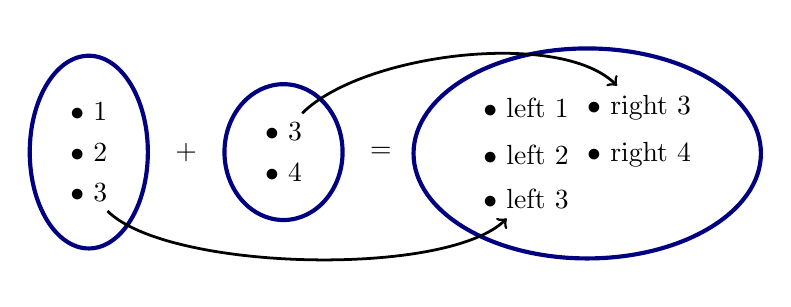
\begin{tikzpicture}
[node distance=5mm,  
 set/.style={line width=1.5pt, shape=ellipse, draw=black!50!blue}]
\matrix [row sep=.5mm] (setA)
{\node (aa) {$\bullet $ 1} ; \\
\node  (ab) {$\bullet $ 2}; \\
\node  (ac) {$\bullet $ 3};\\
};
\node[set,minimum size=1.5cm,fit={(aa) (ac)}] {};
\node [right=of setA] (plus) {$+$};
\matrix [row sep=.5mm, right=of plus] (setB)
{\node (b1) {$\bullet $ 3} ; \\
\node  (b2) {$\bullet $ 4}; \\
};
\node[set,minimum size=1.5cm,fit={(b1) (b2)}] {};
\node [right=of setB] (equal) {$=$};
\matrix [row sep=.5mm, right=of equal, xshift=3mm, ampersand replacement=\&] {
\node  (ca1) {$\bullet$ left 1}; \& \node  (ca2) {$\bullet$ right 3};\\
\node  {$\bullet$ left 2}; \& \node  (cb2) {$\bullet$ right 4};\\
\node  (cc1) {$\bullet$ left 3}; \& \node (cc2) {};\\
};
\node[set,minimum size=1.5cm,fit={(ca1) (cc1) (cb2) (cc2)}] {};
\draw [line width=1pt,->] (ac) .. controls +(1,-1) and +(-1,-1) .. (cc1);
\draw [line width=1pt,->] (b1) .. controls +(1,1) and +(-1,1) .. (ca2);
\end{tikzpicture}
\item $\#(S + T) = $\pause $\#S + \#T$
\item C \texttt{union}'s are disjoint union?
\end{itemize}
\end{frame}

\defverbatim[colored]\codeuniC{%
\begin{lstlisting}[language={C}]
union number { double real; int integer; } x;
\end{lstlisting}}
\defverbatim[colored]\codeunisecC{%
\begin{lstlisting}[language={C}]
x.real=3.14; printf("%d\n",x.integer);
\end{lstlisting}}
\defverbatim[colored]\codeuniH{
\begin{lstlisting}[language={Haskell}]
data Number = RealVal Float | IntVal Int | Rational (Int,Int)
x = Rational (3,4)
y = RealVal 3.14
z = IntVal 12    {-- You cannot access different values --}
\end{lstlisting}}

\begin{frame}
\begin{itemize}
 \item  \textbf{C:} int + double:
 \begin{beamercolorbox}{cexample}
 \codeuniC
\end{beamercolorbox}
\item C \texttt{union}'s are not safe! Same storage is shared. Valid field is unknown:
\begin{beamercolorbox}{cexample}
 \codeunisecC
\end{beamercolorbox}
\item \textbf{Haskel:} Float + Int + (Int $\times$ Int):
\begin{beamercolorbox}{hexample}
 \codeuniH
\end{beamercolorbox}
\end{itemize}
\end{frame}

\section{Mappings}
\begin{frame}
 \frametitle{Mappings}
\begin{itemize}
 \item The set of all possible mappings
 \item $S \mapsto T = \{ V \mid \forall (x \in S) \exists (y \in T), (x \mapsto y) \in V \}$ 
\item Example:
$S=\{ a, b \} \;\;\; T=\{ 1, 2, 3\}$\\
%\psframebox[linecolor=blue!50!black,framearc=1.5]{%
%	\begin{tabular}{l}\rnode{a}{$\bullet $a}\\
%		\rnode{b}{$\bullet $b}\end{tabular}} \ \ 
%\psframebox[linecolor=blue!50!black,framearc=1.5]{%
%	\begin{tabular}{l}\rnode{n1}{$\bullet $1}\\
%		\rnode{n2}{$\bullet $2}\\
%		\rnode{n3}{$\bullet $3}\\
%	\end{tabular}}
%\ncarc[linecolor=red,nodesep=2pt]{|->}{a}{n1}
%\ncarc[linecolor=red,nodesep=2pt]{|->}{b}{n2}
%\ncarc[linecolor=blue,nodesep=2pt]{|->}{a}{n2}
%\ncarc[linecolor=blue,nodesep=2pt]{|->}{b}{n3}
%\ncarc[linecolor=green,nodesep=2pt]{|->}{a}{n3}
%\ncarc[linecolor=green,nodesep=2pt]{|->}{b}{n1}
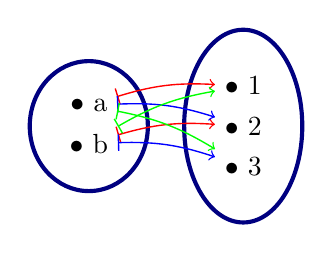
\begin{tikzpicture}
[node distance=5mm,  
 set/.style={line width=1.5pt, shape=ellipse, draw=black!50!blue},
 arrowa/.style={|->,line width=0.5pt,bend left=10,draw=red},
 arrowb/.style={|->,line width=0.5pt,bend left=10,draw=blue},
 arrowc/.style={|->,line width=0.5pt,bend left=10,draw=green}]
\matrix [row sep=.5mm] (setA)
{\node (aa) {$\bullet $ a} ; \\
\node  (ab) {$\bullet $ b}; \\
};
\node[set,minimum size=1.5cm,fit={(aa) (ab)}] {};
\matrix [row sep=.5mm, right=of setA,xshift=5mm] (setB)
{\node (b1) {$\bullet $ 1} ; \\
\node  (b2) {$\bullet $ 2}; \\
\node  (b3) {$\bullet $ 3}; \\
};
\node[set,minimum size=1.5cm,fit={(b1) (b3)}] {};
\draw[arrowa] (aa) to (b1);
\draw[arrowa] (ab) to (b2);
\draw[arrowb] (aa) to (b2);
\draw[arrowb] (ab) to (b3);
\draw[arrowc] (aa) to (b3);
\draw[arrowc] (ab) to (b1);
\end{tikzpicture}%
\hspace{2em}
{\small \begin{minipage}[b]{12em}Each color is a value in the mapping. Other 6 values are not drawn\\[2em]\end{minipage}}\\
{\small $S \mapsto T = \{ 
\{a\mapsto 1, b\mapsto 1\}, 
	{\color{red}\{a\mapsto 1, b\mapsto 2\}}, \{a\mapsto 1, b\mapsto 3\},$\\
$\{a\mapsto 2, b\mapsto 1\}, \{a\mapsto 2, b\mapsto 2\}, 
	{\color{blue}\{a\mapsto 2, b\mapsto 3\}},$\\
${\color{green}\{a\mapsto 3, b\mapsto 1\}},
	 \{a\mapsto 3, b\mapsto 2\}, \{a\mapsto 3, b\mapsto 3\}
\}$}
\item $\#(S \mapsto T) = $\pause  $\#T^{\#S}$
\end{itemize}
\end{frame}

\defverbatim[colored]\codediziP{%
\begin{lstlisting}[language={Pascal}]
type
   Day = (Mon,Tue,Wed,Thu,Fri,Sat,Sun);
   Month = (Jan,Feb,Mar,Apr,May,Jun,Jul,Aug,Sep,Oct,Nov,Dec);
var
   x : array Day of real;
   y : array Month of integer;
...
   x[Tue] := 2.4;
   y[Feb] := 28;
\end{lstlisting}}

\subsection{Arrays}
\begin{frame}
 \frametitle{Arrays}
\begin{itemize}
 \item \texttt{double a[3]=\{1.2,2.4,-2.1\};} \\
	$\mathtt{a} \in (\{0,1,2\} \mapsto \mathtt{double})$ \\
	$\mathtt{a} = (0\mapsto 1.2, 1\mapsto 2.4, 2\mapsto -2.1)$
 \item Arrays define a mapping from an integer range (or DOPT) to any other type
 \item \textbf{C:}
	$T\;\;\mathtt{x}[N]\;\;\Rightarrow\;\; \mathtt{x} \in 
		(\{0,1,..., N-1\} \mapsto T)$
 \item Other array index types (Pascal):
\begin{beamercolorbox}{pexample}
\codediziP
\end{beamercolorbox}

\end{itemize}
\end{frame}

\defverbatim[colored]\codefonkesC{%
\begin{lstlisting}[language={C}]
int f(int a) {
    if (a%2 == 0) return 0;
    else return 1;
}
\end{lstlisting}}
\defverbatim[colored]\codefonkesH{%
\begin{lstlisting}[language={Haskell}]
f a = if mod a 2 == 0 then 0 else 1
\end{lstlisting}}

\subsection{Functions}
\begin{frame}
 \frametitle{Functions}
\begin{itemize}
 \item C function:
\begin{beamercolorbox}{cexample}
\codefonkesC
\end{beamercolorbox}
\item $\mathtt{f}:\mathtt{int} \mapsto \{0,1\}$\\
	regardless of the function body: $\mathtt{f}:\mathtt{int} \mapsto \mathtt{int}$
\item Haskell:
\begin{beamercolorbox}{hexample}
\codefonkesH
\end{beamercolorbox}
\item in C, \texttt{f} expression is a pointer type
	\mbox{\texttt{int (*)(int)}}\\
	in Haskell it is a mapping: \mbox{\texttt{int$\mapsto$int}}
\end{itemize}
\end{frame}

\begin{frame}
 \frametitle{Array and Function Difference}
  \begin{columns}
   \begin{column}{.5\textwidth}
    \structure{Arrays:}
	\begin{itemize}
	 \item Values stored in memory
	 \item Restricted: only integer domain
	 \item \texttt{double$\mapsto$double} ?
	\end{itemize}
   \end{column}
   \begin{column}{.5\textwidth}
    \structure{Functions}
	\begin{itemize}
	 \item Defined by  algorithms
	 \item Efficiency, resource usage
	 \item All types of mappings possible
	 \item Side effect, output, error, termination problem.
	\end{itemize}
   \end{column}
  \end{columns}
\end{frame}

\begin{frame}
\frametitle{Cartesian Mappings}
 \begin{itemize}
  \item Cartesian mappings:\\
	\texttt{double a[3][4];}\\
	\texttt{double f(int m, int n);}
  \item Cartesian mapping versus mappings of mappings:\\
   	\texttt{int$\times$int$\mapsto$double} and \texttt{int$\mapsto$(int$\mapsto$double)}
  \item For cartesian mapping, you need two or more values to get the value of the mapping
  \item In mapping of mappings, you get a new mapping as you supply a value.
 \end{itemize}
\end{frame}

\defverbatim[colored]\codekdizP{%
\begin{lstlisting}[language={Pascal}]
var
   x : array [1..3,1..4] of double;
   y : array [1..3] of array [1..4] of double;
...
x[1,3] := x[2,3]+1;     y[1,3] := y[2,3]+1;
\end{lstlisting}}

\begin{frame}
\frametitle{Cartesian Mapping vs Nested mapping}
\begin{itemize}
 \item Pascal arrays
	\begin{beamercolorbox}{pexample}
	\codekdizP
	\end{beamercolorbox}
\item\ \\
\begin{columns}
 \begin{column}[t]{.45\linewidth}
 Row operations:\\
	\texttt{ y[1] := y[2] ; } {\color{green}$\surd$}\\
	\texttt{ x[1] := x[2] ; } {\color{red}$\times$}
\end{column}
\begin{column}[t]{.5\linewidth}
 \begin{tabular}[t]{|l|l|l|l|}
\multicolumn{4}{l}{\tt x}\\\hline
& & & \\ \hline
& & & \\ \hline
& & & \\ \hline
 \end{tabular}\hspace*{2em}
\begin{tabular}[t]{|l|l|l|l|l|l|}
\multicolumn{6}{l}{\tt y}\\ \cline{1-1}\cline{3-6}
&$\rightarrow$& & & &\\ \cline{1-1}\cline{3-6}
&$\rightarrow$& & & &\\ \cline{1-1}\cline{3-6}
&$\rightarrow$& & & &\\ \cline{1-1}\cline{3-6}
 \end{tabular}
\end{column}
\end{columns}
	
\end{itemize}
\end{frame}

\defverbatim[colored]\codekfonH{%
\begin{lstlisting}[language={Haskell}]
f (x,y) = x+y
g x y = x+y
...
f (3+2)
g 3 2
\end{lstlisting}}

\begin{frame}
 \begin{itemize}
  \item Haskell functions:
\begin{beamercolorbox}{hexample}
\codekfonH
\end{beamercolorbox}
 \item \texttt{g 3}  {\color{green}$\surd$}\\
       \texttt{f 3}  {\color{red}$\times$}\\
 \item Reuse the old definition to define a new function:\\
	\texttt{increment = g 1} \\
	\texttt{increment 1}\\
	\texttt{2}
 \end{itemize}
\end{frame}


\defverbatim[colored]\codekumeP{%
\begin{lstlisting}[language={Pascal}]
type
   color = (red,green,blue,white,black);
   colorset = set of color;
var
   a,b : colorset;
...
a := [red,blue];
b := a*b;                  (* intersection *)
b := a+[green,red];        (* union *)
b := a-[blue];             (* difference *)
if (green in b) then ...   (* element test *)
if (a = []) then ...       (* set equality *)
\end{lstlisting}}


\section{Powerset}
\begin{frame}
 \frametitle{Powerset}
\begin{itemize}
  \item ${\cal P}(S) =  \{ T \mid T \subseteq S \}$
  \item The set of all subsets
  \item\ \\
%$S=$\psframebox[linecolor=blue!50!black,framearc=1.5]{%
%	\begin{tabular}{l}$\bullet $1\\$\bullet $2\\$\bullet $3\end{tabular}}
%\ \ ${\cal P}(S)=$
%\psframebox[linecolor=blue!50!black,framearc=.8]{%
%	\begin{tabular}{l}
%$\bullet \emptyset$\ \ $\bullet \{1\}$\ \  $\bullet \{2\}$\ \ $\bullet \{3\}$\\\ 
%$\bullet \{1,2\}$\ \  $\bullet \{1,3\}$\\
%$\bullet \{2,3\}$\ \ $\bullet \{1,2,3\}$
%	\end{tabular}}
$S = $ 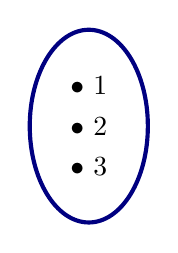
\begin{tikzpicture}
[node distance=5mm,  baseline=(current bounding box.center),
 set/.style={line width=1.5pt, shape=ellipse, draw=black!50!blue}]
\matrix [row sep=.5mm] (setA)
{\node (aa) {$\bullet $ 1} ; \\
\node  (ab) {$\bullet $ 2}; \\
\node  (ac) {$\bullet $ 3}; \\
};
\node[set,minimum size=1.5cm,fit={(aa) (ac)}] {};
\end{tikzpicture}
\hfill
${\cal P}(S) = $ \begin{tikzpicture}
[node distance=5mm, baseline=(current bounding box.center), 
 set/.style={line width=1.5pt, shape=ellipse, draw=black!50!blue}]
\matrix [row sep=.5mm, right=of setA,xshift=5mm, ampersand replacement=\&] (setB)
{\node (aa){$\bullet \emptyset$} ; \& \node {$\bullet \{3\}$};      \& \node (ba){$\bullet \{2, 3\}$}; \\
 \node {$\bullet \{1\}$};      \& \node {$\bullet \{1, 2\}$};   \& \node {$\bullet \{1,2,3\}$}; \\
 \node (ab) {$\bullet \{2\}$} ;  \& \node {$\bullet \{1, 3\}$};\& \node (bb) {};\\
};
\node[set,minimum size=1.5cm,fit={(aa) (ab) (ba) (bb)}] {};
\end{tikzpicture}
  \item $\#{\cal P}(S) = $\pause $2^{\#S}$
\end{itemize}
\end{frame}
\begin{frame}
\begin{itemize}
  \item Set datatype is restricted and special datatype. Only exists in \structure{Pascal} and
  special set languages like \structure{SetL}
  \item set operations (Pascal)
\begin{beamercolorbox}{pexample}
\codekumeP
\end{beamercolorbox}

  \item in \structure{C++} and \structure{Python} implemented as class.
\end{itemize}

\end{frame}

\section{Recursive Types}
\subsection{Lists}
\begin{frame}
 \frametitle{Recursive Types}
\begin{itemize}
 \item $S = ... S ...$
 \item Types including themselves in composition.
\end{itemize}
\structure{\large\bf Lists}
\begin{itemize}
 \item $S = Int \times S + \{null\}$
\[\begin{array}{ll}
S = & \{right\;empty\} \cup \{ left\;(x,empty) \mid x \in Int \} \cup \\
  & \{left\;(x, left\;(y, empty)) \mid x, y \in Int \} \cup \\
  & \{left\;(x, left\;(y, left\;(z,empty))) \mid x,y,z \in Int \} \cup  ...
  \end{array}
\]
\item $S = \{right\;empty, left(1,empty), left(2,empty), left(3,empty), ...,$\\
	$left(1,left(1,empty)), left(1,left(2,empty)), left(1,left(3,empty),...,$\\
	$left(1,left(1,left(1,empty))), left(1,left(1,left(2,empty))), ...\}$
\end{itemize}
\end{frame}

\defverbatim[colored]\codelisteC{%
\begin{lstlisting}[language={C}]
struct List {
     int x;
     List *next;
} a;
\end{lstlisting}}
\defverbatim[colored]\codelisteH{
\begin{lstlisting}[language={Haskell}]
data List = Left (Int,List) | Empty 
     
x = Left (1, Left(2, Left(3,Empty)))  {-- [1,2,3] list --}
y = Empty                             {-- empty list, [] --}
\end{lstlisting}}
\begin{frame}
 \begin{itemize}[<+->]
  \item C lists: pointer based. Not actual recursion.
  \begin{beamercolorbox}{cexample}
   \codelisteC
  \end{beamercolorbox}
\item Haskell lists.
  \begin{beamercolorbox}{hexample}
   \codelisteH
  \end{beamercolorbox}
 \end{itemize}
\end{frame}
\defverbatim[colored]\codecoklisteH{
\begin{lstlisting}[language={Haskell}]
data List alpha = Left (alpha,List alpha) | Empty 
     
x = Left (1, Left(2, Left(3,Empty)))     {-- [1,2,3] list --}
y = Left ("ali",Left("ahmet",Empty))    {-- ["ali","ahmet"] --}
z = Left(23.1,Left(32.2,Left(1.0,Empty))){-- [23.1,32.2,1.0] --}
\end{lstlisting}}
\begin{frame}
 \begin{itemize}[<+->]
  \item Polymorphic lists: a single definition defines lists of many types.
  \item	$List\;\alpha = \alpha \times (List\;\alpha) + \{empty\}$
\begin{beamercolorbox}{hexample}
\codecoklisteH
\end{beamercolorbox}
\item $Left(1,Left(``ali'',Left(15.23,Empty) \in List\;\alpha$ ? \pause
No.\\
	Most languages only permits homogeneous lists.
 \end{itemize}
\end{frame}

\begin{frame}
\frametitle{Haskell Lists}
\begin{itemize}[<+->]
 \item binary operator ``:'' for list construction:\\
	\texttt{data [alpha] = (alpha : [alpha]) | []}
 \item \texttt{x = (1:(2:(3:[])))}
 \item Syntactic sugar:\\
	\texttt{[1,2,3] $\equiv$ (1:(2:(3:[])))}\\
	\texttt{["ali"] $\equiv$ ("ali":[])}
\end{itemize}
\end{frame}

\subsection{General Recursive Types}
\begin{frame}
 \frametitle{General Recursive Types}
\begin{itemize}[<+->]
 \item $T = ... T ...$
 \item Formula requires a minimal solution to be representable:\\
	$S = Int \times S$ \\
	Is it possible to write a single value? No minimum solution here!
 \item List example:\\
	\texttt{x = Left(1,Left(2,x))}\\
	$x \in S$? \pause {\color{green!70!black}Yes} \\
	can we process \texttt{[1,2,1,2,1,2,...]} value?
\item Some languages like \textsf{Haskell} lets user define such values. All iterations go
infinite. Useful in some domains though.
\item Most languages allow only a subset of $S$, the subset of finite values.
\end{itemize}
\end{frame}

\defverbatim[colored]\codeagacC{%
\begin{lstlisting}[language={C++}]
template<class Alpha>
struct Tree {
     Alpha x;
     Tree *left,*right;
} root;
\end{lstlisting}}
\defverbatim[colored]\codeagacH{
\begin{lstlisting}[language={Haskell}]
data Tree alpha = Empty | 
                      Node (alpha,Tree alpha, Tree alpha)
     
x = Node (1,Node (2,Empty,Empty),Node(3,Empty,Empty))
y = Node(3,Empty,Empty)
\end{lstlisting}}


\begin{frame}
 \begin{itemize}[<+->]
  \item $Tree\;\alpha = empty + node\;\alpha\times Tree \alpha \times Tree \alpha$
{\scriptsize
\[\begin{array}{ll}
Tree\;\alpha= & \{empty\} \cup \{node(x,empty,empty) \mid x \in \alpha\} \cup \\
     & \{node(x,node(y,empty,empty),empty) \mid x,y \in \alpha \} \cup \\
     & \{node(x,empty,node(y,empty,empty)) \mid x,y \in \alpha \} \cup \\
     & \{node(x,node(y,empty,empty),node(z,empty,empty)) \mid x,y,z \in \alpha \} \cup ...
  \end{array}
\]
}
\item C++ (pointers and template definition)
\begin{beamercolorbox}{cexample}
 \codeagacC
\end{beamercolorbox}

\item Haskell
\begin{beamercolorbox}{hexample}
 \codeagacH
\end{beamercolorbox}
 \end{itemize}
\end{frame}

\subsection{Strings}
\begin{frame}
\frametitle{Strings}
\begin{itemize}[<+->]
\item Language design choice:
\begin{enumerate}[<+->]
\item Primitive type (ML, Python): \\
	Language keeps an internal table of strings
\item Character array (C, Pascal, ...)
\item Character list (Haskell, Prolog, Lisp)
\end{enumerate}
 \item Design choice affects the complexity and efficiency of:\\
  concatenation, assignment, equality, lexical order, decomposition
\end{itemize}
 \end{frame}

\section{Type Systems}
\begin{frame}
\frametitle{Type Systems}
 \begin{itemize}[<+->]
  \item Types are required to provide data processing, integrity checking, efficiency, access
  controls. Type compatibility on operators is essential.
\item Simple bugs can be avoided at compile time.
\item Irrelevant operations:\\
	\texttt{y=true * 12;\\
	x=12; x[1]=6;\\
	y=5; x.a = 4;}
\item When to do type checking? Latest time is before the operation. Two options:
\begin{enumerate}
 \item Compile time $\rightarrow$ static type checking
 \item Run time  $\rightarrow$ dynamic type checking
\end{enumerate}
 \end{itemize}
\end{frame}

\subsection{Static Type Checking}
\begin{frame}
 \frametitle{Static Type Checking}
\begin{itemize}[<+->]
 \item  Compile time type information is used to do type checking.
 \item All incompatibilities are resolved at compile time. Variables
 	have a fixed time during their lifetime.
\item  Most languages do static type checking
 \item User defined constants, variable and function types:
	\begin{itemize}
	\item Strict type checking. User has to declare all types (C, C++, Fortran,...)
	\item Languages with type inference (Haskell, ML, Scheme...)
	\end{itemize}
 \item No type operations after compilation. All issues are resolved. Direct machine code
 instructions.
\end{itemize}
\end{frame}

\subsection{Dynamic Type Checking}
\begin{frame}[fragile]
 \frametitle{Dynamic Type Checking}
\begin{itemize}[<+->]
 \item Run-time type checking. No checking until the operation is to be executed.
 \item Interpreted languages like Lisp, Prolog, PHP, Perl, Python.
 \item Python:
\begin{beamercolorbox}{pexample}
\begin{lstlisting}[language=Python]
def whichmonth(inp):
    if isinstance(inp, int):
        return inp
    elif isinstance(inp, str):
        if inp == "January":
            return 1
        elif inp == "February":
            return 2
        ....
        elif inp == "December":
            return 12
...
inp = input()     /* user input at run time? */
month=whichmonth(inp)
\end{lstlisting}
\end{beamercolorbox}
\end{itemize}
\end{frame}

\begin{frame}
\begin{itemize}
\item Run time decision based on users choice is possible.
\item Has to carry type information along with variable at run time.
\item Type of a variable can change at run-time (depends on the language).
\end{itemize}
\end{frame}

\begin{frame}
 \frametitle{Static vs Dynamic Type Checking}
\begin{itemize}
 \item Static type checking is \structure{faster}. Dynamic type checking does type checking before each
 operation at run time. Also uses extra memory to keep run-time type information.
 \item Static type checking is more restrictive meaning \structure{safer}. Bugs avoided at compile time,
 earlier is better.
 \item Dynamic type checking is less restrictive meaning more
 \structure{flexible}. Operations working on
 dynamic run-time type information can be defined.
\end{itemize}
\end{frame}


\defverbatim[colored]\codeisimesit{%
\begin{lstlisting}[language={C}]
typedef struct Comp { double x, y;}  Complex;
struct COMP { double x,y; };

struct Comp a;
Complex b;
struct COMP c;

/* ... */
a=b;   /* Valid, equal types */
a=c;   /* Compile error, incompatible types */
\end{lstlisting}}

\subsection{Type Equality}
\begin{frame}
 \frametitle{Type Equality}
\begin{itemize}[<+->]
 \item $S \stackrel{?}{\equiv}  T$  How to decide?
\begin{itemize}
 \item \structure{Name Equivalence}: Types should be defined at the same exact place.
 \item \structure{Structural Equivalence}: Types should have same value set. (mathematical set
 equality).
\end{itemize}
\item Most languages use \structure{name equivalence}.
\item C example:
\begin{beamercolorbox}{cexample}
\codeisimesit
\end{beamercolorbox}
\end{itemize}
\end{frame}

\begin{frame}
 \frametitle{Structural Equality}
$S \equiv T$ if and only if:
\begin{enumerate}
 \item $S$ and $T$ are primitive types and  $S = T$ (same type),
 \item if $S=A\times B$, $T=A'\times B'$, $A \equiv A'$, and $B \equiv B'$,
 \item if $S=A+B$, $T=A'+B'$, and ($A \equiv A'$ and $B \equiv B'$) or
	($A \equiv B'$ and $B \equiv A'$ ),
 \item if $S=A\mapsto B$, $T=A'\mapsto B'$, $A \equiv A'$ and $B \equiv B'$,
 \item if $S={\cal P}(A)$, $T={\cal P}(A')$, and $A \equiv A'$.
\end{enumerate}
Otherwise $S \not\equiv T$
\end{frame}

\defverbatim[colored]\codeisimcev{%
\begin{lstlisting}[language={C}]
enum Day {Mon, Tue, Wed, Thu, Fri, Sat, Sun} x;
x=3;
\end{lstlisting}}

\begin{frame}
 \begin{itemize}[<+->]
  \item Harder to implement structural equality. Especially recursive cases.
  \item $T = \{nil\} +A\times T\;,\;\;T' = \{nil\} + A\times T'$ \\ \pause
	$T = \{nil\} +A\times T'\;,\;\;T' = \{nil\} + A\times T$ 
  \item \texttt{struct Circle \{ double x,y,a;\};} \\
	\texttt{struct Square \{ double x,y,a;\};} \\
	Two types have a semantical difference. User errors may need less tolerance in such
	cases.
 \item Automated type conversion is a different concept. Does not necessarily conflicts with name
 equivalence.
\begin{beamercolorbox}{cexample}
\codeisimcev
\end{beamercolorbox}
 \end{itemize}
\end{frame}

\section{Type Completeness}
\begin{frame}
 \frametitle{Type Completeness}
\begin{itemize}[<+->]
 \item First order values:
	\begin{itemize}
	\item Assignment
	\item Function parameter
	\item Take part in compositions
	\item Return value from a function
	\end{itemize}
 \item Most imperative languages (Pascal, Fortran) classify functions as second order value. (C
 represents function names as pointers)
 \item Functions are first order values in most functional languages like Haskell and Scheme .
 \item Arrays, structures (records)?
 \item \structure{Type completeness principle:} First order values should take part in all
 operations above, no arbitrary restrictions should exist.
\end{itemize}
\end{frame}

\def\OK{\color{green!60!black}$\surd$}
\def\NO{\color{red!60!black}$\times$}

\rowcolors[]{2}{blue!10}{blue!5}

\begin{frame}

C Types:\\
{\scriptsize
\begin{tabular}{>{\bf}lcccc} \rowcolor{blue!20} 
			&\bf	Primitive& \bf Array& \bf Struct&\bf Func. \\
Assignment			&	\OK	& \NO	& \OK	& \NO	\\
Function parameter 	&	\OK	& \NO	& \OK	& \NO	\\
Function return		&	\OK	& \NO	& \OK	& \NO	\\
In compositions		&	\OK	&\tikz[remember picture,overlay] \node (no3) {\OK} ; 
						& \OK	& \NO	\\
\end{tabular}}\\[1.5em]


Haskell Types:\\ \rowcolors[]{2}{green!10}{green!5}
{\scriptsize
\begin{tabular}{>{\bf}lcccc} \rowcolor{green!20} 
			&\bf	Primitive& \bf Array& \bf Struct&\bf Func. \\
Variable definition	& \OK	& \OK	& \OK	& \OK \\
Function parameter 	&	\OK	& \OK	& \OK	& \OK	\\
Function return		&	\OK	& \OK	& \OK	& \OK	\\
In compositions		&	\OK	& \OK	& \OK	& \OK	\\
\end{tabular}
}\\[1.5em]


Pascal Types:\\ \rowcolors[]{2}{red!10}{red!5}
{\scriptsize
\begin{tabular}{>{\bf}lcccc} \rowcolor{red!20} 
			&\bf	Primitive& \bf Array& \bf Struct.&\bf Func. \\
Assignment		&	\OK	& \OK	& \OK	& \NO	\\
Function parameter 	&	\OK	& \OK	& \OK	& \NO	\\
Function return		&	\OK	& \tikz[remember picture,overlay] \node (no1) {\NO} ;
					& \tikz[remember picture,overlay] \node (no2) {\NO} ;
							& \NO	\\
In compositions		&	\OK	& \OK	& \OK	& \NO	\\
\end{tabular}
\begin{tikzpicture} [remember picture,overlay] 
\node [draw=red,circle,thick,fit=(no1),inner sep=0pt] {};
\node [draw=red,circle,thick,fit=(no2),inner sep=0pt] {};
\node [draw=red,circle,thick,fit=(no3),inner sep=0pt] {};
\end{tikzpicture}
}
\end{frame}

\section{Expressions}
\begin{frame}
\frametitle{Expressions}
 Program segments that gives a value when evaluated:
\begin{itemize}
	\item Literals
	\item Variable and constant access
	\item Aggregates
	\item Variable references
	\item Function calls
	\item Conditional expressions
	\item Iterative expressions (Haskell)
\end{itemize}
\end{frame}

\subsection{Literals/Variable and Constant Access}
\begin{frame}
\frametitle{Literals/Variable and Constant Access}
\begin{itemize}
 \item \structure{Literals}: Constants with same value with their notation\\
 \texttt{123, 0755, 0xa12, 12451233L, -123.342,}\\
\texttt{ -1.23342e-2, 'c', \path{'\021'}, "ayse", True, False}
 \item \structure{Variable and constant access}: User defined constants and variables give their
 content when evaluated.\\
\texttt{int x; }\\
\texttt{\#define pi 3.1416}\\
\texttt{\textsf{x}=\textsf{pi}*\textsf{r}*\textsf{r}}
\end{itemize}
\end{frame}

\defverbatim[colored]\codeaggH{
\begin{lstlisting}[language={Haskell}]
x=(12,"ali",True)              {-- 3 Tuple --}
y={name="ali", no=12}	       {-- record   --}
f=\x -> x*x                    {-- function --}
l=[1,2,3,4]                    {-- recursive type, list --}
\end{lstlisting}}
\defverbatim[colored]\codeaggC{
\begin{lstlisting}[language={C},escapechar=\#]
struct Person { char name[20], int no };
struct Person p = {"Ali Cin", 332314};
double arr[3][2] = {{0,1}, {1.2,4}, {12, 1.4}};
p={"Veli Cin",123412}; #\NO# /* not possible in ANSI C!*/
\end{lstlisting}}
\defverbatim[colored]\codeaggCnn{
\begin{lstlisting}[language={C},escapechar=\#]
int (*arr)[2]; 
arr = {{0, 1}, {1.2,4}, {12, 1.4}}; #\OK#
p = (struct person) {"Veli Cin",123412}; #\OK# /* C99 */
\end{lstlisting}}

\subsection{Aggregates}
\begin{frame}[fragile]
\frametitle{Aggregates}
\begin{itemize}
 \item Used to construct composite values without any declaration/definition.
 Haskell:
\begin{beamercolorbox}{hexample}
 \codeaggH
\end{beamercolorbox}
 \item Python:\\
\begin{beamercolorbox}{pexample}
\begin{lstlisting}
 x = (12, "ali", True)
 y = [ 1, 2, [2, 3], "a"]
 z = { 'name':'ali', 'no':'12'}
 f = lambda x:x+1
\end{lstlisting}
\end{beamercolorbox}
\end{itemize}
\end{frame}

\begin{frame}[fragile]
\begin{itemize}
\item Ansi C has aggregates \structure{only} at the
definition. There is no aggregates in the statements!
\begin{beamercolorbox}{cexample}
 \codeaggC
\end{beamercolorbox}
\item C99 \structure{Compound literals} allow array and structure aggragates
\begin{beamercolorbox}{cexample}
 \codeaggCnn
\end{beamercolorbox}
\item C++11 has function aggragetes (lambda)\\
\begin{beamercolorbox}{cexample}
\begin{lstlisting}
void sort(int a[], int n, (*f)(int,int)) {
	...
}
auto f = [](int a) { return a+1;} ;
...
sort(arr, n, [](int a, int b) { return a-b;});
n = f(n)
\end{lstlisting}
\end{beamercolorbox}
\end{itemize}
\end{frame}

\subsection{Variable References}
\begin{frame}
\frametitle{Variable References}
\begin{itemize}
\item Variable access vs variable reference
\item value vs l-value
\item \alert{pointers are not references!} You can use pointers as references with special
operators.
\item Some languages regard references like first order values (Java, C++ partially)
\item Some languages distinguish the reference from the content of the variable (Unix shells,
ML) 
\end{itemize}
\end{frame}

\subsection{Function Calls}
\begin{frame}
\frametitle{Function Calls}
 \begin{itemize}
  \item $F (Gp_1, Gp_2, ..., Gp_n) $
  \item Function name followed by actual parameter list. Function is called, executed and the
  returned value is substituted in the expression position.
  \item \structure{Actual parameters:} parameters send in the call
  \item \structure{Formal parameters:} parameter names used in function definition
  \item Operators can be considered as function calls. The difference is the infix notation.
  \item $\oplus (a,b)$ vs $a \oplus b$ 
  \item languages has built-in mechanisms for operators. Some languages allow user defined
  operators (operator overloading): C++, Haskell.
 \end{itemize}
\end{frame}

\defverbatim[colored]\codecondC{
\begin{lstlisting}[language={C}]
x = (a>b)?a:b;
y = ((a>b)?sin:cos)(x);     /* Does it work? try yourself... */
\end{lstlisting}}

\subsection{Conditional Expressions}
\begin{frame}
\frametitle{Conditional Expressions}
 \begin{itemize}[<+->]
  \item Evaluate to different values based on a condition.
  \item Haskell: \texttt{if {\em condition\/} then {\em exp1\/} else {\em
  exp2\/}}  .\\
	\hspace*{2em}\texttt{case {\em value\/} of  {\em p1\/} -$>$ 
		{\em exp1\/} ; {\em p2\/} -$>$ {\em exp2\/} ...}
  \item C: \texttt{({\em condition\/})?{\em exp1\/}:{\em exp2 \/}; }
\begin{beamercolorbox}{cexample}
\codecondC
\end{beamercolorbox}
  \item Python: \texttt{{\em exp1\/} if {\em condition\/} else {\em exp2\/}}
  \item \texttt{if .. else} in C is \alert{not} conditional expression but
  conditional statement. No value when evaluated!
\end{itemize}
\end{frame}

\defverbatim[colored]\codecondH{
\begin{lstlisting}[language={Haskell}]
x = if (a>b) then a else b
y = (if (a>b) then (+) else (*)) x y
data Day = Mon | Tue | Wed | Thu | Fri | Sat | Sun
convert a = case a of
          Left (x,rest) -> x : (convert rest)
          Empty -> []
daynumber g = case g of 
          Mon -> 1
          Tue -> 2
          ...
          Sun -> 7
\end{lstlisting}}

\begin{frame}
 \begin{itemize}
  \item Haskell:
\begin{beamercolorbox}{hexample}
 \codecondH
\end{beamercolorbox}
\item \texttt{case} checks for a pattern and evaluate the RHS expression
with substituting variables according to pattern at LHS.
 \end{itemize}
\end{frame}

\defverbatim[colored]\codeiterH{
\begin{lstlisting}[language={Haskell}]
x = [1,2,3,4,5,6,7,8,9,10,11,12]
y = [ a*2 | a <- x ]               {-- [2,4,6,8,...24 ] --}
z = [ a | a <- x, mod a 3 == 1 ]   {-- [1,4,7,10] --}
\end{lstlisting}}

\defverbatim[colored]\codeiterP{
\begin{lstlisting}[language={Python}]
x = [1,2,3,4,5,6,7,8,9,10,11,12]
y = [ a*2  for a in x ]             #  [2,4,6,8,...24 ] 
z = [ a for a in x if a % 3 == 1 ]  #  [1,4,7,10]
z = { a:a*a for a in x}             #  {1:1,4:16,7:49,10:100}
\end{lstlisting}}

\subsection{Iterative Expressions}
\begin{frame}
 \frametitle{Iterative Expressions}
\begin{itemize}
 \item Expressions that do a group of operations on elements of a list or
 data structure, and returns a value.
 \item \texttt{[ {\em expr\/} \path{|} {\em variable\/} $<$- {\em list\/}
 , {\em condition\/}]}
 \item Similar to set notation in math:\\
	 $\{ expr | var \in list, condition \}$
\item Haskell:
\begin{beamercolorbox}{hexample}
\codeiterH
\end{beamercolorbox}
\item Python:
\begin{beamercolorbox}{pexample}
\codeiterP
\end{beamercolorbox}
\end{itemize}

\end{frame}

\subsection{Block Expressions}
\begin{frame}[fragile]
 \frametitle{Block Expressions}
\begin{itemize}
\item Some languages allow multiple/statements in a block to calculate a value.
\item GCC extension for compound statement expressions:\\
\begin{beamercolorbox}{cexample}
\begin{lstlisting}
double s, i, arr[10];
s = ( { double t = 0; 
        for (i = 0; i < 10; i++)
            t += arr[i];
        t;}) + 1;    
\end{lstlisting}
\end{beamercolorbox}
Value of the last expression is the value of the block.
\item ML has similar block expression syntax.
\item This allows arbitrary computation for evaluation of the expression.
\end{itemize}
\end{frame}

\section{Summary}
\begin{frame}
\frametitle{Summary}
\begin{itemize}
\item Value and type
\item Primitive types
\item Composite types
\item Recursive types
\item When to type check
\item How to type check
\item Expressions
\end{itemize}

\end{frame}



\end{document}
